\chapter{Introduction}
\label{sec:intro}
\begin{summary}
  In this work I discuss a modification of a fluorescence microscope    \cma{my device}
  that minimizes the toxic effects of the excitation light.

  In the following introductory chapter I describe what phototoxicity   \cma{phototoxicity}
  is and how it comes about. Then I give an example of how it
  influences biological observations in a developing \celegans\ 
  embryo and describe how this particular biological system can be
  used to evaluate and compare the phototoxicity of different microscopes.

  Later in this chapter I give an overview of image formation   \cma{cameras}
  in the wide-field microscope and I describe its principle limitations
  regarding resolution and depth discrimination. Furthermore I
  discuss the two most important current image detector technologies
  --- electron multiplying charge-coupled devices (EMCCD) and
  scientifc complementary metal–oxide–semiconductor (sCMOS).
\end{summary}
\nomenclature{EM-CCD}{Electron multiplying charge-coupled devices}
Regardless of whether it is the picture of earth captured by an
orbiting satellite, the x-ray motion picture of a running dog or the
time-lapse recording of a blooming flower. Images capture our
imagination and they are a good starting point to develop new models
and theories.

This is particularly true for microscopy.  Only after people became
aware of microorganisms by direct observation, medieval quack could
finally be overcome and modern medicine based on the scientific
method flourished instead.

Even today --- with electron microscopes, magnetic resonance
tomography and sequencing machines --- optical microscopy still is an
indispensable tool for research of living organisms.

Fluorescence microscopy is of particular importance: It enables the     \cma{labelling, switching}
scientist to selectively label a particular type of molecule in living cells
and observe how they perform their biological function.

Besides localizing molecules it is possible to measure physical
quantities inside of the sample. There are, for example, fluorescent
labels that report membrane potentials or viscosity inside of cells.

Finally, it is even possible to exert a controlling function with the
excitation light: There are compounds that locally release chemicals
when illuminated and there are  genetically encoded ion channels that can be
switched by light \citep{Boyden2005}.

However, the excitation light introduces unnatural and potentially
deleterious energy into the specimen. If the exogenous light harms the
observed organism in any way, this effect is called phototoxicity.

% dennoch: from photophysical prospective of single- and multi-photon
% microcopy, probably the most disheartening reality is the occurrence
% of photobleaching and photodamage
% \citep{diaspro2009nanoscopy}

There are a number of techniques that can reduce phototoxicity: Two
photon excitation, controlled light exposure, selective plane
illumination, highly inclined and laminated optical sheet, and oblique
plane microscopy. I introduce them in
chapter \ref{sec:illum-patterns}. These techniques have different
pros and cons and not all are equally suited for a specific problem,
e.g.\ selective plane illumination is very effective, but it needs two
perpendicular lenses and can not be used for multiwell plates or to
observe the liver of a living, adult mouse.

In this work I present an approach that makes use of modern display
and camera technology. We only modify the microscope's illumination
path, the space around objective lens and specimen remains as
accessible as in any conventional wide-field microscope.



\section{Phototoxicity in life sciences and the model organism
  \celegans}
\label{sec:intro-phototoxicity}
The partner in our project who is responsible for decisions related to
life sciences and biology is Institut Pasteur (Paris, FR). They work
on infectious diseases. 

In order to motivate the importance of phototoxicity, I would like to
portray an elegant drug screening experiment which I have seen on one
of my visits in Paris: An automatic microscope continuously images a
cell culture in multiwell plates. These cells carry a pathogen. The
pathogen, the nuclei of the cultured cells and the membranes of the
cells are each stained with a different fluorophore. The cells in each
well of the plates are exposed to a different chemical.

A chemical is considered a hit and will be investigated during further
trials, when the time lapse images show that the culture cells stay
healthy and the number of pathogens decrease. As neither people nor
animals come to harm, this screening experiment is an impeccable
method to systematically understand and hopefully heal certain
diseases. However, this experiment does not work very well, if the
excitation light --- and not the drug --- kills the pathogens. The
effect of phototoxicity should therefore be minimized.


Now one would hardly develop a microscope and directly test it with
dangerous pathogens. As part of our collaboration, the Institut
Pasteur therefore developed a safe biological test system that is
relatively easy to maintain \citep{Stiernagle2006} and allows to test
the phototoxicity of various microscopes \citep{Tinevez2012}.




The basis of the system is the embryo of the organism \celegans. These
are small invertebrates. The adult form is approximately \unit[1]{mm}
long.  Their anatomy and development are comparatively simple and have
been well characterized \citep{Sulston1977,Durbin1987}.

\jpginput{12cm}{celegans-devel}{Phototoxic effects while imaging the
  embryonal development of three \celegans\ embryos (strain
  AZ212, histone-2B tagged with eGFP) with different excitation
  intensities. The embryo with lowest excitation dosage (left)
  develops fastest. The embryo with the highest dosage (right) ceases
  development and nearly all fluorophores are bleached after the
  experiment. Images by J.-Y. Tinevez (Institut Pasteur, Paris, FR).}
  

We use embryos of a genetically modified strain\footnote{Our strain
  has WormBase ID AZ212 \citep{Praitis2001}.} that expresses eGFP
tagged histones (enhanced green fluorescent protein, excitation
maximum \unit[488]{nm}, emission maximum \unit[509]{nm}). Histones are
incorporated into the chromatin during cell divisions, i.e.\ the
nuclei of our worms fluoresce green.  The mother worm passes a
sufficient amount of these proteins into the cytoplasm of the
embryo. In the beginning of its development the embryo entirely relies
on this reserve of histones. Only in a much later stage --- certainly
not during the first few hours, that we observe --- it will form its
own histones.

\figref{fig:celegans-devel} compares time-lapse experiments on three \cma{embryo example} 
different \celegans\ embryos with varying
excitation intensities.

The lineage tree of two developing \celegans\ embryos is the \cma{reproducible development}
same.  With all other factors being equal, particularly if the
temperature is constant at $\unit[21\pm
1]{\degreeCelsius}$, two different embryos will develop at the
same speed from egg to fertile adult in three and a half days.


At the beginning of the experiment, embryos are removed from their
mothers at an identical stage, before any cellular divisions have
occured. Then a $z-$stack of the egg with 41 slices and one micron
$z-$sampling is obtained every two minutes.

The columns in \figref{fig:celegans-devel} depict three different embryos
whose development was imaged according to this protocol for two hours
and 38 minutes with different excitation powers.

The figure displays the maximum intensity projections of the
$z-$stacks.  In order to make the cell nuclei visible in all images, I
normalized the data to the same range. As can be guessed from the
photon shot noise, the upper left image contains the least number of
fluorescence photons, and the upper right the most.

An analysis of the time-lapse data show that one hour into the
experiment the embryo with the highest excitation dose (right) has
stopped developing and its fluorophores are strongly bleached.  Some
cells even turned apoptotic and went into programmed cell death.

After two hours and 38 minutes the experiment was stopped and the
embryo which was exposed to the lowest dose (left) has developed the
largest number of cells. The middle embryo ceased developing while the
right embryo died even earlier and nearly all its fluorophores are
bleached at the end of the experiment.

In \figref{fig:worm-integration-time} I reproduce quantitative data
from \cite{Tinevez2012}. Each data point in this graph corresponds to
a two hour time-lapse imaging experiment of a \celegans\ embryo in a
wide-field microscope. From a very low excitation up to a certain
threshold dose the development is not affected by the light and
approximately 50 cells develop during the two hours.

For a dose above the threshold the development is slowed due to
phototoxicity and the number of cells at the end of the experiment
decreases.

\gnuplotinput{worm-integration-time}{Longer exposure times are less
  phototoxic. Each data point corresponds to one embryo that developed
  under a particular excitation dose for two hours. The solid lines
  are sigmoidal fits to the data. Also indicated are the two
  phototoxicity thresholds given by the inflection point of the
  sigmoid and their $95\%$ confidence intervals. This data was
  provided by J.-Y. Tinevez (Institut Pasteur, Paris, FR) and is also
  published in \cite{Tinevez2012}.}  

The orange data points in the diagram correspond to a per slice
integration time $\tau$ of \unit[100]{ms} and for the green data
the integration time is five times higher.

\nomenclature{$\Omega$}{Excitation dose in $\joule/(\centi\meter^2\textrm{stack})$} 
\nomenclature{$\Phi_e$}{Radiant flux of excitation light in watts} 
The dose $\Omega$ on the $x-$axis is calculated as
\begin{align}
\Omega = \frac{\Phi_e n \tau}{A},
\end{align}
with integration time $\tau$, area $A$ of the illuminated field, the
number of slices $n=41$ and radiant flux $\Phi_e$ of the excitation
light, as measured in the pupil.

Naively one would assume that it should not make any difference if the
excitation light dose is administered with \unit[100]{ms} or
\unit[500]{ms} exposures but these data show that a longer exposure
time and low intensity are less phototoxic.

These results agree with an earlier study in tobacco plants
\citep{Dixit2003}. They investigate cell death a few days after
illumination and find that there is a threshold dose below which no
phototoxicity can be detected, and that this threshold decreases with
light intensity. Dixit and Cyr show that the damage is caused by
reactive oxygen species and they explain the shift of the
phototoxicity threshold by the limited capacity of the cells'
scavenging system for those radicals. They also predict the existence
of redox-sensitive checkpoints in the mitotic division cycle.

%\citep{Sancar2004}

In summary this section describes how to measure phototoxicity with
biological specimen.  The next section gives an overview of the
underlying photophysics and the rest of this work describes our
attempt to build a microscope with reduced phototoxic footprint.



\section{Photophysical principles of phototoxicity}
\label{sec:photophysics}
\begin{summary}
  Here I give a short overview of fluorescence of molecules in order
  to introduce the terms photobleaching and phototoxicity.
\end{summary}
A fluorophore is a molecule that can absorb and subsequently emit
light. During the absorption of a photon the molecular orbital
transitions from the electronic ground state $S_0$ to an excited state
$S_1$. The lifetime of the excited state $S_1$ is in the order of a
few nanoseconds.
\begin{figure}[!hbt]
  \centering
  \svginput{.8}{flu-level}
  \caption{The Jablonski energy level diagram of an illustrative
    fluorescent molecule. The boxes depict orbitals, up and down
    arrows symbolize the spin of the outer electrons. Fat horizontal
    lines represent electronic states. Thinner lines indicate
    vibro-rotational states. Various processes are shown with their
    typical time scales. VR = vibro-rotational relaxation, ISC =
    intersystem crossing, IC = internal conversion \cite[inspired
    from][]{Haken2006}.}
  \label{fig:flu-level}
\end{figure}
A Jablonski diagram, as depicted in \figref{fig:flu-level}, summarizes
information \cma{energy levels} about the energy levels of a molecule
and possible transition processes.

%  If the photon has an even higher
% energy, the electron will go into the second excited singlet state
% $S_2$.

The majority of known stable and bright fluorophores absorb and emit
in the wavelength range between \unit[300]{nm} and \unit[700]{nm}.
Photons at the high energy end of this range can excite molecules into
higher energy levels $S_n, (n>1)$ than the first excited state; these
states are unstable and hardly return to the ground state $S_0$. On
the other side of the spectrum: a molecule that absorbs in the
near-infrared ($\unit[>700]{nm}$) has a low-lying excited singlet
state $S_1$ and therefore potentially increased reactivity and a high
probability for a non-radiative transfer back into the ground state
$S_0$ \citep{Sauer2011}.


The term \emph{Stokes' shift} describes the frequency shift between
the absorbed and emitted photon; the energy difference is lost as heat
to the fluorophore molecule and surrounding solvent.  For the
practical implementation of fluorescence microscopes this is
significant, as it enables to separate excitation and emission light
with a dichroic beam splitter.


The excitation probability of a fluorescence molecule depends on the
orientation of its dipole axis relative to the plane of vibration of
the excitation field. Especially if the molecule is not rigidly bound
to a bigger structure or embedded in a viscous solvent it will
reorient its dipole during the fluorescence lifetime and emit the
fluorescence photon in a random direction. We use this in the next
section to describe image formation in the fluorescence microscope.


The triplet states $T_n$ play an important role in photobleaching.
Pure electronic absorption of one photon has no effect on the spin of
an electron and therefore the transition from singlet states $S_n$
into the triplet state $T_n$ should not occur. However, interaction
with the nuclei can mediate this spin transition. Therefore, in
fluorophores this transition has a small probability, resulting in
long lifetimes of the triplet state $T_1$.

\cite{Deschenes2002} show that excitation of higher triplet states
$T_n$ is the predominant reactive process for photobleaching in
vacuum. In particular they measured that one rhodamine~6G molecule
\emph{in vacuum} can emit more than \num{1e9} photons before it
bleaches, if the excitation intensity is low enough
$(\sim\unit[1]{\si{\watt/\cm^2}})$ to prevent decay over triplet
states.

In normal atmosphere the prolonged lifetime of the triplet state $T_1$
makes it highly likely for the fluorophore to react with molecular
oxygen $\O_2$. Oxygen is abundant and has a triplet ground state
${}^3\Sigma$ with two unpaired electrons of parallel spin in its
$\pi^*-$orbitals (see \figref{fig:oxygen}).

  \citep{Bernas2004}

\begin{figure}[!hbt]
  \centering
  \svginput{1}{oxygen}
  \caption{{\bf left:} Schematic that depicts how the orbitals of the
    oxygen molecule are formed from the atomic orbitals. {\bf right:}
    Molecular oxygen has the lowest energy in its triplet state
    ${}^3\Sigma$ where the spins of the two outer $\pi^*-$electrons
    are parallel. Inspired from \citet{Linde2011a}.}
  \label{fig:oxygen}
\end{figure}

If a ground-state oxygen molecule comes into physical contact with a
$T_1$ fluorophore, the energy of the latter can be transferred by an
electron exchange energy transfer mechanism in which the orbitals
directly interact with each other \citetext{\citealp[p.~438]{Haken2006} and
  \citealp{Linde2011a}}.

During this reaction, which is also known as triplet--triplet
annihilation, two forms of singlet oxygen form in competition: The
lower energy state ${}^1\Delta$ and the short-lived, higher energy
state ${}^1\Sigma$ that immediately ($T_{1/2}\sim\unit[10^{-9}]{s}$)
sends out a \unit[1268]{nm} photon and decays into ${}^1\Delta$.

The resulting singlet oxygen ${}^1\Delta$ is very reactive. In a
typical specimen it diffuses only a few tens of nanometres until it
reacts with another molecule.

(FIXME 2000 greenbaum measures oxygen production, bernas 2004 anoxia gfp)

Nowadays many methods are known to reduce photobleaching: Substitute
oxygen with noble gases or remove it enzymatically
\citep[p.~89]{Sauer2011}, depopulate the triplet state by adding
reducing as well as oxidizing agents to the solvent
\citep{Vogelsang2008} or couple a triplet quencher directly to the
fluorophore \citep[p.~19]{Sauer2011}. For fixed samples it helps to
change the solvent or polymer.
 
In living specimen these techniques may reduce photobleaching, but
they can also have a detrimental effect on the biological system
itself. Removing oxygen will quite certainly have a negative
effect. In order to reduce phototoxicity it makes sense to think about
the light management in the microscope.


\section{Conventional microscopes}
\begin{summary}
  The wide-field fluorescence microscope does not excite fluorophores
  of the specimen in an optimal way. In this section I outline how
  these microscopes work and explain how out-of-focus blur severely
  limits their performance. I introduce the terms point spread
  function, optical transfer function and etendue.
\end{summary}

\subsection{Ray-optical description of a large-aperture lens}

A microscope, is a device that collects light coming from one plane  \cma{lateral image}
and forms a magnified image on a
camera. \figref{fig:widefield-microscope}~b) shows a schematic
representation of the detection path of a wide-field microscope.

The main components are an objective lens with focal length $f$ and a
\cma{telecentricity} tube lens TL1 with focal length
$f_\textrm{TL}>f$. Sample, lenses and camera are arranged in
double-telecentric configuration, i.e.\ the sample is located in the
front focal plane of the objective, the tube lens is at distance
$f_\textrm{TL}$ behind the pupil (i.e.\ the back focal plane of the
objective) and the camera is in the focal plane behind the tube lens.


\nomenclature{$\beta$}{Transversal magnification of an objective
  $\beta=f_\mathrm{TL}/f$, for Zeiss lenses the magnification $\beta$
  is written on the objective and the focal length of the tube lens is
  defined as $f_\textrm{TL}=\unit[164.5]{mm}$}


Light from the sample is collimated by the objective lens and
\cma{lateral magnification} re-imaged by the tube lens. The lateral
magnification $\beta$ is given by the ratio of the focal lengths of
the two lenses:
\begin{align}
  \beta=\frac{\overline{O'P'}}{\overline{OP}}=\frac{f_\mathrm{TL}}{f}.
\end{align}
Note that in \figref{fig:widefield-microscope}~b) I represent the
objective lens as a single element.  This is a simplification.

In the paraxial limit ray-tracing calculations for a thick lens or
even several consecutive lens elements can be simplified by bending
the ray only at one place --- at the principal plane.

\nomenclature{marginal ray}{Axial ray through the periphery of the
  entrance aperture}

\nomenclature{chief ray}{Ray from the periphery of the field through
  the center of the entrance aperture}

\nomenclature{entrance aperture}{Projection of the limiting aperture
  of the optical system into object space}


Microscope objectives must collect light from a large aperture in
\cma{perfect imaging and high-aperture} order to produce a high
resolution image. This is a fact I will support shortly using the
wave-optical model. Unfortunately the large ray angles in the
objective prevent its simplified description using principal planes,
but an analysis using the eikonal theory \citep{Haferkorn1984} shows % page 125 2.3.2 mikroobjektive65g ggggg g gg g v g      v  v--*


that an optical system that fulfills the Abbe sine condition allows
perfect imaging even for widespread ray bundles.
\begin{align}
  \label{eq:sine-condition}
  \beta = \frac{n \sin\alpha}{n' \sin\alpha'} \qquad \textrm{(Abbe sine condition)}
\end{align}
This condition ensures that the focal length, a quantity which is
usually defined only for paraxial rays, is equal for all angles.  This
in turn means that such a lens carries out a Fourier transform from
the front to the back focal plane with linear scaling. Note that a
lens with a non-linear distortion in the back focal plane will fail to
produce an image that is similar to the object.

It turns out that ray bending in a high-aperture lens system that  \cma{aplanatic sphere}
fulfills the Abbe sine condition can be simplified to a one bend at a
single surface, quite similar to the utilization of principal planes
in paraxial optics. For a high-aperture system this surface is no
longer a plane.  Instead it is a sphere with radius $n f$ and called
\emph{aplanatic sphere}. I depict this surface as two circle segments
with bold red strokes on the lenses in
\figref{fig:widefield-microscope}~b).

In addition to the Abbe sine condition microscope lenses are also
corrected for spherical aberration and linear coma \citep{Gross2005}.
Then the coma rays are symmetric around the chief ray, the wavefront
and point spread function are approximately invariant for small field
sizes (in first order).  This ensures that the imaging conditions are
invariant for small regions of the field plane and allows to express
image formation with linear systems theory.

\subsection{Wave-optical theory for image formation in a fluorescence microscope}
In the following I want to describe how the image on the camera
\cma{wave optics} is formed. For this we have to use wave theory because
close to the image rays intersect, invalidating ray-optical
predictions. As both, wave-optical and ray-optical theory, are very
much related, we can give a useful interpretation of the aplanatic
surface for wave optics.

The underlying Maxwell equations and the wave equation are linear and   \cma{plane waves}
we can represent propagating solutions (evanescent solutions are
neglected) of the wave equation as a superposition of the elementary
solution --- the monochromatic, plane waves described by wave vector
$\k$:
\begin{align}
  u(\r,t)=u\,\exp(i(\k\r-\omega t)),\quad \r=(r_x,r_y,r_z),\
  \k=(k_x,k_y,k_z),\ |\k|=2\pi \underbrace{n/\lambda_0}_{1/\lambda},
\end{align}
with vacuum wavelength $\lambda_0$, refractive index $n$ and
wavelength $\lambda$ in the immersion medium.

The accurate treatment of high-aperture optics would in fact require a
vectorial calculation of the image for a fluorophore with a particular
dipole orientation.  Subsequently these images should be averaged to
account for random fluorophore orientations, but as I do not need
quantitative expressions I limit myself to the simpler scalar problem
which provides qualitatively similar results.
% \begin{figure}[!hbt]
%   \centering
%   \svginput{1}{sine-condition}
%   \caption{dasfklj}
%   \label{fig:sine-condition}
% \end{figure}

\begin{figure}[!hbt]
  \centering
  \svginput{1}{widefield-microscope}
  \caption{{\bf a)} Segment of the three-dimensional frequency
    spectrum of the light from the sample that is collected by the
    objective lens is highlighted in red on the Ewald sphere. {\bf b)}
    Schematic of the detection path of a modern microscope. The sample
    is in the front focal plane of the objective. The detection tube
    lens TL1 forms a magnified image on the camera. The aplanatic
    spheres for objective and tube lens are indicated in
    \textcolor{red}{red}. {\bf c)} Parallel laser epifluorescence
    excitation. The excitation tube lens TL2 focuses a laser into the
    pupil of the objective. The beam is reflected by a dichroic beam
    splitter (BS) towards the objective. An extended area in the
    specimen is illuminated. Fluorescence light returns through the
    objective, is transmitted through BS and forms an image on the
    camera. }
  \label{fig:widefield-microscope}
\end{figure}
Assuming that the excited fluorophores in the sample give rise to a
\cma{Ewald sphere} monochromatic electromagnetic field --- I simplify
the problem by omitting the complication that fluorophores emit
photons in a wavelength range --- then using the spatial frequency
vector $\vnu=\k/(2\pi)$ we can expand the three-dimensional,
stationary field amplitude distribution $u(\r)$ into its spatial
frequency spectrum $\widetilde u(\vnu)$:

\nomenclature{$u(\r)$}{Scalar field as a function of spatial
  coordinates} 

\nomenclature{$\widetilde u(\vnu)$}{Fourier transform
  of scalar field as a function of spatial frequencies}

\nomenclature{$\r=(r_x,r_y,r_z)^T$}{Three-dimensional spatial
  coordinate} 

\nomenclature{$\r_t=(r_x,r_y)^T$}{Transversal two-dimensional spatial
  coordinate}

\nomenclature{$\vnu=(\nu_x,\nu_y,\nu_z)^T$}{Three-dimensional spatial
  frequency}

\nomenclature{$\vnu_t=(\nu_x,\nu_y)^T$}{Transversal two-dimensional
  spatial frequency}


\begin{table}[!hbt]
  \centering
  \begin{tabular}{ l l | l }
    $u(\r):$&$ \mathbb{R}^3\to\mathbb{C}$ & field distribution in sample space \\
    $u'(\r'):$&$\mathbb{R}^3\to\mathbb{C}$ & field distribution in image space \\
    $S(\r):$ & $\mathbb{R}^3\to\mathbb{R}$ & distribution of fluorophores in sample space \\
    $I'(\r'):$&$\mathbb{R}^3\to\mathbb{R}$ & intensity distribution in image space\\
    $\widetilde u(\vnu):$&$\mathbb{R}^3\to\mathbb{C}$ & spatial frequency spectrum of field in sample space \\
    $a(\r):$&$\mathbb{R}^3\to\mathbb{C}$ & amplitude point spread function \\
    $\widetilde a(\vnu):$&$\mathbb{R}^3\to\mathbb{C}$ & amplitude transfer function, generalized aperture \\
    $h(\r)=|a(\r)|^2:$&$\mathbb{R}^3\to\mathbb{R}$ & intensity point spread function \\
    $\widetilde h(\vnu):$&$\mathbb{R}^3\to\mathbb{C}$ & optical transfer function \\
  \end{tabular}
  \caption{Overview of the functions that are used in this section.}
  \label{tab:widefield-functions}
\end{table}



\begin{align}
  u(\r)=\mathcal{F}(u(\vnu)):=\int_{-\infty}^{\infty}\int_{-\infty}^{\infty}\int_{-\infty}^{\infty}
  \widetilde u(\vnu) \exp(2\pi i \r\vnu)\ \textrm{d}^3 \vnu
\end{align}
Where $\mathcal{F}$ denotes the Fourier transform operation. I will
use several functions in this section. See
Table~\ref{tab:widefield-functions} for a listing of their names.

Since we have assumed a monochromatic field and the length $|\vnu|$ of
the spatial frequency vector is the inverse of the wavelength
($n/\lambda_0$, in the material of refractive index $n$), the support
(denoted '$\supp$') of this spectrum $\widetilde u(\vnu)$ is limited
to the surface of a sphere of radius $n/\lambda_0$:
\begin{align}
  \supp \widetilde u(\vnu) &= \{\vnu \in \mathbb{R}^3: |\vnu|=n/\lambda_0\}.
\end{align}
This sphere is the transfer function of free space, and is also called
Ewald sphere.  \nomenclature{Ewald sphere}{Transfer function of free
  space} Scaling the Ewald sphere with $f\lambda_0$ gives the
aplanatic surface of the lens. Note that the $x-$component of the
marginal ray (in the $xz-$plane) corresponds to the spatial frequency
component $\nu_x = n\sin\alpha$ in object space and
$\nu_x'=n'\sin\alpha'$ with $n'=1$ in image space. The transversal
spatial frequency components are related due to the Abbe sine
condition (\ref{eq:sine-condition}):
\begin{align}
  \beta &= \nu_x/\nu_x',\quad  \beta = \nu_y/\nu_y'.
\end{align}
The transfer function $\widetilde a(\vnu)$ of the lens is defined by
complex values on the Ewald sphere \citep{McCutchen1964}:
\begin{align}
  \widetilde a(\vnu)&=P(\vnu_t) \exp\left(\frac{2\pi i}{\lambda} 
    W(\vnu_t)\right)
  \delta\left(|\vnu|-\frac{n}{\lambda_0}\right)  \step(\nu_z),\\
  \step(x)&=
  \begin{cases} 
    1 & x\ge 0 \\
    0 & x<0 
  \end{cases}, \qquad \textrm{(Heaviside step function)} \label{eq:unit-step}
\end{align}
with the Dirac delta function $\delta$, transversal spatial frequency
vector $\vnu_t=(\nu_x,\nu_y)^T$, and the real valued pupil function
$P(\vnu_t)$ and wavefront error $W(\vnu_t)$. McCutchen calls the
three-dimensional function $\widetilde a(\vnu)$ the generalized
aperture.

For this discussion I set $W(\vnu_t)=1$, i.e.\ there is no wavefront
aberration and the lens is diffraction limited. Furthermore, I use a
uniform, solid cylinder as pupil function $P(\vnu_t)$ in order to
limit the size of the calotte (or cap) of the Ewald sphere that is
defined by the acceptance angle $\alpha$ of the
objective\footnote{Note that this expression is only valid for
  $\alpha\in[0,\pi/2]$. An expression for $\widetilde a(\vnu)$
  encompassing the full range $[0,\pi]$ for $\alpha$ must contain two
  functions of each $P$ and $W$, in dependence on whether the spatial
  frequency vector $\vnu$ is directed in or against the direction of
  the optical axis. This is necessary to express the transfer function
  of a 4Pi or I${}^n$M microscope.}:

% \begin{align}
%   \widetilde a(\vnu) =
%   \begin{cases}
%     P_-(\vnu_t) \exp\left(\frac{2\pi i}{\lambda} 
%     W_-(\vnu_t)\right)
%   \delta\left(|\vnu|-\frac{n}{\lambda_0}\right) & \nu_z<0
%  \\
% P_+(\vnu_t) \exp\left(\frac{2\pi i}{\lambda} 
%     W_+(\vnu_t)\right)
%   \delta\left(|\vnu|-\frac{n}{\lambda_0}\right) & \nu_z\ge 0
%   \end{cases}
% \end{align}

\begin{align}
  P(\vnu_t) &=
  \step\left(|\vnu_t|-\frac{n\sin(\alpha)}{\lambda_0}\right), 
\end{align}
with the Heaviside step function as defined in equation
(\ref{eq:unit-step}.  In general $P(\vnu_t)$ can assume values between
0 and 1 in order to account for apodization due to natural vignetting
or angle-dependent Fresnel reflection losses on the lenses. I ignore
such effects in this discussion. Also, just as the objective lens, the
tube lens can be described by its generalized aperture but I assume
that the tube lens maintains a diffraction limited wavefront of the
full angular range. For this discussion, the full microscope is
readily described by the generalized aperture of just its objective
lens.

Multiplication of the angular frequency spectrum $\widetilde u(\vnu)$
with the generalized aperture $\widetilde a(\vnu)$ gives the angular
frequency spectrum of the amplitude in the image:
\begin{align}
  \widetilde u'(\vnu') = \widetilde u'(\vnu/\beta) = \widetilde u(\vnu/\beta)\cdot \widetilde a(\vnu/\beta).
\end{align}
Note that I use the transversal magnification $\beta$ to scale the
arguments of the functions, so that the result is given in image space
spatial frequencies\footnote{Unfortunately my notation is slightly
  problematic here. I assume that $z-$sampling occurs by stepping the
  sample through the object space while the camera is fixed in the
  focal plane of the tube lens. Therefore the axial coordinates $r_z$
  and $r'_z$ in object and image are identical.}.

According to the convolution theorem this multiplication in frequency
space corresponds to a convolution in the domain of spatial
coordinates $\r$ of the field distribution $u(\r)$ and an amplitude
point spread function $a(\r)=\mathcal{F}(\widetilde a(\vnu))$ that
describes the imaging of the objective lens:
\begin{align}
  u'(\r')=u'(\beta \r) = (u \otimes a)(\r) =
  \int_{-\infty}^{\infty}\int_{-\infty}^{\infty}\int_{-\infty}^{\infty}
  u(\vvarrho)\ a(\r-\vvarrho)\ \textrm{d}^3\vvarrho
\end{align}
where $\vvarrho$ is a spatial coordinate and the lateral magnification
$\beta=\r'/\r$ transforms between image space $\r'$ and object space
$\r$. This result shows that the three-dimensional amplitude
distribution of the image is linearly related to the amplitude
distribution in the sample.

A focal plane detector can only measure the intensity $I'$ which
depends non-linearly on the amplitude of the field $u'$.  However, the
fluorophores act as independent sources and their phases vary randomly
with respect to each other. Each fluorophore gives rise to its
coherent image $h(\r')$  \citep{goodman1968}:
\begin{align}
  h(\r')=|a(\r')|^2.
\end{align}
The three-dimensional intensity distribution $I'(\r')$ in image space
can then be obtained by incoherently adding the individual images of
the fluorophores:
\begin{align}
  I'(\r') &= \int_{-\infty}^{\infty}\int_{-\infty}^{\infty}\int_{-\infty}^{\infty}
  S(\vvarrho)\ h(\r'-\vvarrho)\ \textrm{d}^3\vvarrho\\
  &= (S \otimes h) (\r')
\end{align}
where $S(\vvarrho)$ represents the three-dimensional fluorophore
distribution and $\vvarrho$ is the spatial coordinate in image space.

It is useful to discuss the Fourier transform of the intensity point  \cma{optical transfer function}
spread function $h$. This is the three-dimensional optical transfer
function of the microscope and describes how well different spatial
frequencies are transmitted:
\begin{align}
  \widetilde h(\vnu') = \mathcal{F}(a(\r')\ a^*(\r')) =
  \widetilde a(\vnu') \otimes \widetilde a^*(-\vnu'). \label{eq:otf}
\end{align}
The product of the amplitude point spread function $a(\r')$ and its
complex conjugate corresponds to an auto-correlation of the amplitude
transfer function in spatial frequency space. Note that the complex
conjugation of the second factor $a^*(\r')$ results in an inversion of
the argument of $\widetilde a^*(-\vnu')$.

This expression allows a geometric interpretation of the support of
the optical transfer function $\widetilde h(\vnu')$
\citep{Gustafsson1995}. Equation (\ref{eq:otf}) describes a
convolution of two spherical caps whose open sides are facing each
other. The entire covered volume somewhat resembles a torus with
vanishing internal diameter. \figref{fig:missing-cone} depicts a
$\nu_x\nu_z-$cross-section for two different aperture angles $\alpha$.
\begin{figure}[!hbt]
  \centering
  \svginput{1}{missing-cone}
  \caption{Schematic depicting $\nu_x\nu_z-$cross sections of the
    support of optical transfer function $\widetilde{h}$ for
    microscope objectives with different collection angles. {\bf
      left:} Objectives, that only collect light that is directed into
    one half space, have the missing cone problem. {\bf right:}
    Optical transfer function for fictional objective with larger
    collection angle and no missing cone.}
  \label{fig:missing-cone}
\end{figure}
The lateral $\Delta\nu_x$ and axial $\Delta\nu_z$ extent of the  
optical transfer function can be expressed in terms of wavelength
$\lambda_0$, immersion index $n$ and aperture angle $\alpha$:
\begin{align}
  \Delta\nu_x =
  \begin{cases}
4 n \sin(\alpha)/\lambda_0 & 0\le \alpha\le \pi/2\\
4 n/\lambda_0 & \pi/2<\alpha<\pi
  \end{cases}
, \quad
  \Delta\nu_z = 2\frac{n}{\lambda_0}(1-\cos\alpha),
\end{align}
(FIXME verify with rainers book chapter) allow to give lower bounds for  \cma{resolution}
the resolution that can be obtained using a well corrected objective: 
\begin{align} 
\label{eq:resolution}
  \Delta d_x = \frac{2}{\Delta\nu_x} = \frac{\lambda_0}{2 n \sin\alpha}, \quad
  \Delta d_z = \frac{2}{\Delta\nu_z} = \frac{\lambda_0}{n(1-\cos\alpha)}.
\end{align}
In order to sample the bandwidth limited signal in the image plane
correctly, the pixel pitch $p_x$ of the camera must be smaller than
half of the resolution: $p_x<\beta\Delta d_x/2$ (Nyquist criterium). A
similar relation holds true for the $z-$sampling: $p_z<\Delta
d_z/2$. Too large a sampling period will result in aliasing artifacts.

Note that the axial resolution $\Delta d_z$ is substantially worse
than the lateral resolution $\Delta d_x$ in normal microscope with a
collection aperture $\alpha<\pi/2$ that is restricted to only one
half-space.

Additionally the optical transfer function of such a microscope is
empty in a cone shaped region around the axis above and below the
origin.  This means that in a conventional wide-field microscope it is
impossible to bring into focus a (defect-free) fluorescent plane
because low spatial frequencies do not attenuate with defocus
\citep{Neil1997}. This effect is also called ``missing cone problem''
\citep{Streibl1984}.

It is instructive to look at a microscope, that is not hampered by the
missing cone problem: In image interference microscopy (I${}^2$M) two
opposing microscope objectives collect light from the sample and the
two detection beam paths are brought to interference using a beam
splitter on a focal plane detector. This configuration substantially
increases the collection angle, improves the $z-$resolution and fills
the missing cone but puts stringent requirements on the optical path
difference between the two interferometer arms, i.e.\ this device is
very sensitive to sample-induced aberrations and in practice, with
fluorophores that emit in a broad wavelength range, this method only
works for samples which are only a few microns thick
\citep{Gustafsson1999}.

\nomenclature{I${}^2$M}{Image interference microscopy
  \citep{Gustafsson1999}.}


Light from the focal plane interferes constructively on the detector,
light emitted at $\lambda/4$ distance away from the focal plane
interferes destructively, light that is emitted at several wavelengths
distance from the focal plane contributes as an incoherent sum to the
detected signal. Therefore a $z-$stack of a fluorescent plane captured
with two opposing lenses compared to just one lens will give a signal
that is four times as bright in focus, shows damped oscillations
(because of the finite spectral band emitted by the fluorophores) when
going away from focus and has twice the brightness out-of-focus. This
means the axial location of the fluorescent plane can be measured in
I${}^2$M but there is still background signal \citep{Gustafsson1995}.

The reason for this background signal is conservation of energy from
plane to plane. A light ray that started in a certain object point
does not stop in the corresponding image point. Therefore most
out-of-focus light is added incoherently as a background to the
detected signal. Structured illumination can be used to remove this
out-of-focus light (FIXME reference to confocal and structured
illumination sections).


\subsection{Illumination in a wide-field epifluorescence microscope}
As mentioned in section \ref{sec:photophysics}, fluorescence photons
are essentially emitted in all directions by a typical, (nearly)
independent of the original illumination direction. Therefore it is
possible and convenient to use the objective for excitation as well as
detection. This mode of microscopy is called epifluorescence (Greek:
$\varepsilon\pi\iota$; on, above).  In this configuration usually only
a small percentage of the excitation light returns due to scattering
or reflection. This simplifies the separation of fluorescence light
from excitation light and parts of opaque specimen can be imaged.

The blue beam in \figref{fig:widefield-microscope}~c) depicts a
parallel laser that is focused into the pupil of the objective by tube
lens TL2. The beam is reflected at a dichroic beam splitter (BS). This
is a glass plate that has been coated with dielectric layers. The
refractive index, thickness and sequence of the layers are designed so
that the excitation light is reflected towards the
objective. Excitation light, that is scattered or reflected in the
sample and returns through the objective is reflected towards the
light source. However, lower energy fluorescence light returning from
the objective is transmitted towards the camera. Behind the objective
the beam is parallel and illuminates the specimen. The field of view
is the demagnified diameter of the laser beam before TL2.

\subsubsection*{Non-uniformity due to coherent interference}
Note that tiny dirt particles in the excitation beam path can cause
coherent interference and produce unwanted non-uniformities in the
illumination. As a remedy the spatial coherence of the laser is
sometimes reduced.  Incoherent light emitting diodes, mercury or xenon
arc lamps are often used instead of lasers. In the latter case a band
pass filter selects the useful part of the spectrum of the excitation
lamp upstream of the dichroic beam splitter.

\subsubsection*{The space-bandwidth product of a microscopic lens}
\label{sec:etendue}
A useful quantity in optics is the etendue $\mathcal{E}$. For a \cma{etendue}
microscope objective its value is related to the number of point spread
functions that can be resolved in the field.  Therefore this quantity
is also called information capacity, light gathering capacity or
space-bandwidth product. For a high-aperture lens, the etendue is
given by \nomenclature{$\mathcal{E}$}{Etendue, information capacity,
  light gathering capacity or space-bandwidth product; its value is
  related to the number of point spread functions that can be resolved
  in the field.}
\begin{align}
\label{eq:high-aperture-etendue}
  \mathcal{E}=\frac{\pi}{4}\left(D_\textrm{field}\,\textrm{NA}\right)^2,
\end{align}
with the numerical aperture $\textrm{NA}$ and the field diameter
$D_\textrm{field}$. The typical image diameter for Zeiss microscopes
is \unit[25]{mm}.  For a $63\times$ oil-immersion objective with
$\textrm{NA}=1.4$ this corresponds to a field diameter of
$D_\textrm{field}=\unit[0.4]{mm}$ and an etendue of
$\mathcal{E}=\unit[0.27]{mm^2/sr}$, where '\unit[]{sr}' denotes
steradian, the SI unit of solid angle.


\subsection{Phototoxicity in conventional microscopes}
When imaging living specimen we should distinguish between useful and
unnecessary excitation. Taking into account the detection capabilities
of objective lenses we should maximize the ratio of in-focus to
out-of-focus fluorescence. The epifluorescent wide-field and confocal
microscope surely do not represent an optimum in this regard.

In chapter \ref{sec:approaches} I will introduce other microscopy
techniques that are more considerate of where to deposit excitation
power within the specimen.

\subsection{Conclusion}
\label{sec:widefield-conclusion}
In this section I introduced a theoretical model that describes image
formation in a wide-field microscope. For well-corrected,
diffraction-limited lenses this process is linear in intensity and
three-dimensionally shift-invariant. In order to predict the image of
a three-dimensional sample it is sufficient to know the image of a
single point source.

By investigating this point spread function and its Fourier transform
it is possible to give the simple relationships in equations
(\ref{eq:resolution}) for the best possible resolution. Furthermore I
describe the missing cone problem, a limitation inherent in all lenses
that only collect light from one half-space.



\section{Image detectors in wide-field microscopy}
\label{sec:ccd-intro}
\begin{summary}
- decribe ccd

- characterization/calibration

- zahlen die ich nenne entsprechen CCDs die ich benutze

- noise

- compare with scmos
\end{summary}

\subsection{Introduction}
Nowadays, all wide-field microscopes use silicon-based cameras to
measure \cma{detection} and digitize the intensity distribution in the
intermediate image plane. The semiconductor surface is patterned with
a two-dimensional array of PIN photodiodes that generate and collect
an intensity-dependent amount of free charge carriers when their
depletion region is exposed to light photons.

Modern detectors can have a very high probability of a photon being
\cma{quantum efficiency and back-thinning} absorbed and contributing to final signal
(quantum efficiency $Q_E$). For the most light sensitive devices even
the backside of the silicon substrate is removed until the diodes can
be exposed from the backside. In this way, the diodes can cover the
entire surface and the fill factor is not reduced due to opaque wires
running over the surface. Such detectors are called 'back-thinned' and
can achieve a quantum efficiency of up to $95\%$ for green light.

There are basically two different technologies to measure and digitize
the charge that was collected in the photodiodes:

In the passive-pixel sensor columns of diodes form a linear row of
\cma{Charge-coupled devices (CCD)} capacitors. By applying a sequence
of different voltages, in the range up of to \unit[6]{V} to each of
three adjacent capacitors, the charge can be transported line by line
out of the sensor --- therefore, this technology is known as
charge-coupled device (CCD). An additional row of similar capacitors
(denoted horizontal shift register) on one side of the array pushes
the carriers into a charge amplifier. \cma{charge amplifier} This
consists of a much smaller capacitor (the read node) and a
field-effect transistor that amplifies the voltage across the read
node. This voltage linearly depends on the charge \citep{Pawley2006}.

In the active-pixel sensor each individual photodiode is surrounded by
its own \cma{active-pixel sensor} transistors for readout and
reset. The two-dimensional array is addressed with an access
enable wire which is shared by pixels of a line and an output wire,
which is shared by pixels of a column. In the simplest case (with
three in-pixel transistors) start of integration and readout occurs
one line at a time (rolling shutter).

When I started this work in 2008, passive CCD sensors were state of
the art detectors for fluorescence microscope with regards to
sensitivity and speed. Now, however, faster and cheaper active-pixel
sensors that provide comparable or better noise performance, become
commercially available.

In the next section I will deal with various noise sources that affect
the signal of focal plane detectors. This is not only relevant to
compare the performance of cameras from different manufacturers or to
determine the optimal parameter settings for one particular
experiment; often it is advantageous to specify an intensity
measurement as the number of detected photoelectrons, e.g.\ when
comparing images of different microscope systems (confocal, spinning
disk or wide-field) or when utilizing sophisticated noise reduction
algorithms.

\subsection{Photon shot noise and read noise}
Fluorescence photons arrive at the \cma{Photon shot noise} detector
independently of each other. This random process leads to fluctuations
in the number of the detected photons and can be described by the
Poissonian probability mass function (denoted as '$\pois$'):
\begin{align}
  \pois(k;\lambda) = \frac{\lambda^k \exp(-\lambda)}{k!},\quad \lambda\in\mathbb{R},\quad k=0,1,2,\ldots
\end{align}
Note that in this particular formula the quantities have a different
meaning than in other parts of this work. The variable $k$ describes
the number of measured photons and the real number $\lambda$ is the
average number of photons that reach the detector during the
integration time. \figref{fig:pois} displays the discrete detection
probabilities for three different values of $\lambda$.

\gnuplotinput{pois}{Poissonian probability mass function
  $\pois(k;\lambda)$ for three photon fluxes with different average
  photon numbers $\lambda$.}


We can calibrate every detector in order to specify the measurement in
the unit of detected photoelectrons. For this, we utilize the property
of the Poisson distribution that the variance $(\Delta I)^2$ of an
intensity measurement (in the unit of photoelectrons) is equal to the
average intensity $\langle I\rangle$:
% nice proof: http://www.proofwiki.org/wiki/Variance_of_Poisson_Distribution
\begin{align}
\label{eq:variance}
  (\Delta I)^2 = \langle(I - \langle I \rangle) ^2\rangle = \langle I\rangle.
\end{align}
\newcommand{\comment}[2]{#2}
\begin{figure}
  \centering
  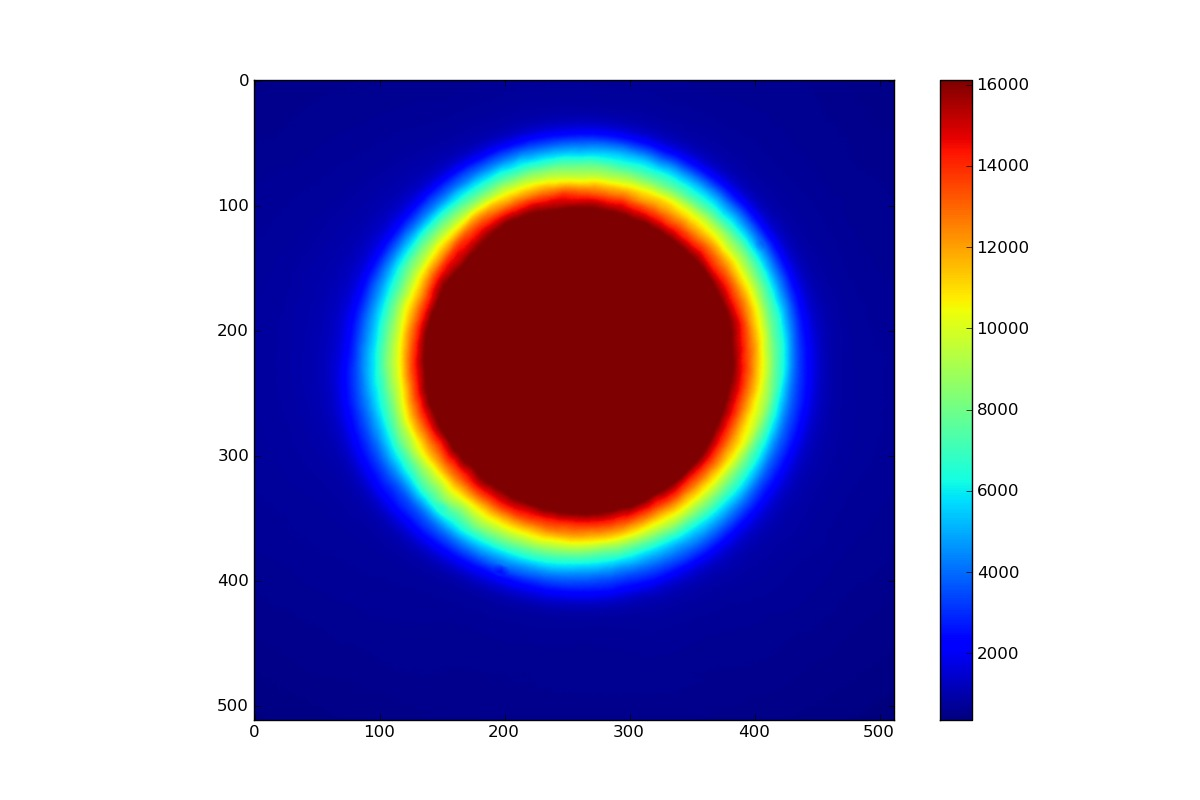
\includegraphics[height=5.9cm, trim=130 10 120 20, clip]{calib-pic}
  \pdfinput{7.4cm, trim=0 0 30 20, clip}{andor_normal_preamp5_exp30}
  \caption{{\bf left:} Image of a defocused area on a fluorescent
    plane sample. This is used for calibrating the detector. {\bf
      right:} Result of a detector calibration. The slope of the curve
    allows to convert the arbitrary analog-to-digital units into
    detected photoelectrons, the point of interception at the $y-$axis
    gives the detector read noise.}
  \label{fig:shot-noise}
\end{figure}
For the calibration of a detector, twenty images of a \cma{detector
  gain calibration} defocused fluorescent object (see left image in
\figref{fig:shot-noise}) are acquired. From the twenty images the
variance of the intensity is determined for each pixel. Then all
occurring intensities are collected into 100 bins. The average
intensity variance of each bin is then plotted against the intensity
(see right image in \figref{fig:shot-noise}). The data lie on a
straight line. From its slope we calculate the gain to convert the
arbitrary analog-to-digital units into the number of detected
photoelectrons. If the data is plotted in this unit, the slope of the
line is one, according to equation \eqref{eq:variance}. The smooth
light distribution in the input images ensures a good coverage for
each data point in the variance-intensity plot. 

\comment{ % this is just for copying the jpeg file
\jpginput{10cm}{calib-pic}{Image of a defocused area on a fluorescent
  plane sample.}}

To determine the quality of a detector we \cma{measuring read noise}
ensure that no light falls on the detector and create twenty dark
images.  For an ideal, noise-free detector these images would contain
zero everywhere. In a real CCD sensor the variance of the values in
the dark images reflect the readout noise $N_r$. Using the calibration
gain, the readout noise can be specified as photoelectrons$/$pixel
(\unit[]{e/px}).

The analysis for the right diagram in \figref{fig:shot-noise} gave a
readout noise of \unit[5.6]{e/px}. For the evaluation I used the
function \verb!cal_readnoise! of the DIPimage toolbox for Matlab
\citep{Lidke2005a}. In appendix \ref{sec:python-readnoise-eval} I list
an alternative Python implementation of this algorithm.

The major source for readout noise is the charge amplifier. Its noise is
added uniformly to every image pixel. For readout frequencies above
\unit[1]{MHz} the readout noise increases with the square root of the
read speed \citep{Pawley2006}. Until a decade ago this limited the
readout speed of scientific CCD cameras. Then a new type of sensor was
developed --- the electron-multiplying CCD (EM-CCD) \citep{Mackay}.

This device contains an additional sequence of capacitors (denoted        \cma{electron-multiplying CCD}
multiplication registers), which are operated with a high voltage (up
to \unit[46]{V}). The field accelerates electrons and they can
generate more charge carriers by a process called impact
ionization. This is a statistical process and for every electron going
through a multiplication register, there is an average probability $p$
that it creates another electron. This probability is quite low
($p<1.3\%$) but after a sequence of 536 registers the gain
$M=(1+p)^{536}\approx 1015$ is so high, that even readout noise at \unit[17]{MHz}
readout speed can be neglected.

This amplification process consumes a lot of energy and requires an
elaborate cooling scheme of the detector chip as the gain is
temperature dependent.

Unfortunately, the statistical nature of impact ionization leads to an
uncertainty in gain and therefore introduces a \cma{excess noise
  reduces quantum efficiency} new noise source. As a gain this noise
acts multiplicately on the signal. \cite{Robbins2003} analyzed the
amplification process and shows that the multiplicative noise, which
is also called excess noise, has the effect of halving the apparent
quantum efficiency of the detector.

Note that for very low light conditions with a minute probability to
detect more than one photon per pixel, the EM-CCD can be run with
maximum gain as a binary detector in photon counting mode. In this
mode the excess noise has no effect whatsoever; but other noise
sources become important.

\newcommand{\SNRid}{\textrm{SNR}_{id}}
\newcommand{\SNRadd}{\textrm{SNR}_{add}}
\newcommand{\SNR}{\textrm{SNR}}
\subsection{Comparison chart for detector selection}
Now I will introduce a comparison chart that I first saw in
\cite{Cameras2012}. It is based on a single formula for the
signal-to-noise ratio $\SNR$ and if the detector parameters, such as
readout noise and quantum efficiency, are known, a quantitative
estimate of the expected quality of the data can be made.

Shot noise defines the fundamental limit for the signal-to-noise ratio
in photo detectors \citep{Sheppard2006a}. As already mentioned above,
the expected noise for a signal of $S$ photons is $\sqrt{S}$. Assuming
the contributions to a detector pixel are $S$ photons signal perturbed
by an additional number of $I_b$ photons background light. The
signal-to-noise $\SNRid$ ratio for an ideal, noise-free detector is:
\begin{align}
  \SNRid = \frac{S}{\sqrt{S+I_b}}.
\end{align}
A conventional detector with reduced quantum efficiency $Q_E\in[0,1]$ and
additive readout noise $N_r$ (in \unit[]{e/px}) can only produce a
worse signal-to-noise ratio:
\begin{align}
  \SNRadd = \frac{Q_E\cdot S}{\sqrt{Q_E(S+I_b)+N_r^2}}.
\end{align}
This formula can be adapted for the electron-multiplying CCD. There,
the readout noise is reduced because of the gain $M$ but the influence
of the shot noise is doubled due to the excess noise factor
$F_n=\sqrt{2}$.
\begin{align}
  \SNR = \frac{Q_E\cdot S}{\sqrt{F_n^2\cdot Q_E \cdot (S+I_b) + (N_r/M)^2}}
\end{align}
This equation makes it possible to compare all the cameras that I can
use for my experiments. Table \ref{tab:cam-param} lists their
parameters and the three diagrams in \figref{fig:camera-snr} shows
curves of the relative signal-to-noise ratio $\SNR/\SNRid$ for three
different amounts of background light $I_b$.
\begin{savenotes}
  \begin{table}[!htbp]
    \centering
    \begin{tabular}{l r r r r r l}
      camera type & $f_\textrm{read}$  & $QE$ & $N_r$ & $F_n$ & $M$ & model \\
       & [MHz] & &  [e/px] & &  &  \\
      \hline
      back-thinned CCD & 1 & 0.95 & 6 & 1 & 1 &  E2V CCD97\\
      EM-CCD & 10 & 0.95 & 9 & $\sqrt{2}$ & 5 and 20 & E2V CCD97 \\
      EM-CCD single photon & 10 & 0.95 & 9 & 1 & 50 & E2V CCD97 \\
      sCMOS global shutter& 200 &0.52 & $2.3$ & 1 & 1 & Fairchild CIS2521F\\
      sCMOS rolling shutter& 140 &0.72 & $1.3$ & 1 & 1 & Hamamatsu FL-400\\
      back-thinned sCMOS & --- &0.95 & $0.7$ & 1 & 1 & --- \footnote{Back-thinned sCMOS are not available at the time of writing.} \\
      interline CCD & 20 & 0.62 & 6.5 & 1 & 1 & Sony ICX285\\
      interline CCD & 1 & 0.62 & 2.4 & 1 & 1 & Sony ICX285\\
    \end{tabular}
    \caption{Camera parameters for the curves in \figref{fig:camera-snr}.}
    \label{tab:cam-param}
  \end{table}
\end{savenotes}

For a very large number of photons the detector with the highest
quantum efficiency $Q_E$ wins (back-thinned CCD, green line):
\begin{align}
  \lim_{S\rightarrow\infty} \frac{\SNR}{\SNRid} &=
  \frac{\sqrt{Q_E}}{F_n}. \qquad \textrm{(high light limit)}
\end{align}
For detectors with readout noise, there is a signal photon number
$S_n$ below which the readout noise predominates:
\begin{align}
  F_n^2 Q_E (S+I_b) &> \frac{N_r^2}{M^2} \\
  S_n&= \frac{N_r^2}{M^2F_n^2 Q_E}-I_b.  \qquad\textrm{(photon shot noise limit)}
\end{align}
I indicate both limits in \figref{fig:camera-snr} using different
line types. The line is dotted in the region where the readout noise
dominates, followed by a thick solid line where both photon shot noise
and readout noise contribute. A thin line indicates the region where
the relative SNR is within 95\% of the high light limit and the
detection is limited by the photon shot noise.


\gnuplotinput{camera-snr}{Camera snr. dotted line for lowest light
  level, where $N_r$ is the dominant noise; thin line indicates high
  light region where quantum efficiency and excess noise factor $F_n$ matter
}
 


The sensor E2V CCD97($512\times512$, pixel pitch \unit[16]{$\mu$m}) is
used in several of our EM-CCD cameras. It has a \citep{2004e2v}
% which is in our EM-CCD cameras Andor IXon2 (head:
% DU-897E-CS0-\#BV) and Photometrics Cascade~II


\cma{interpretation of \figref{fig:camera-snr}}


- effects to look out for

- signal pickup fft of dark image to see periodic offset fluctuations

- gain fluctuations have multiplicative influence more of a problem for scmos

- not clear how frequent recalibration will be required


- heating during read can lead to offset drift

- make sure all the charge is transported out

- light source brightness fluctuation

- room light


- Higher gains are possible but limit the dynamic range.

- maximum charge handling capacity with linear response: 400000 \citep{2004e2v}


- cic is a problem

- thermal effects lead to generation of charge in a ccd

- for long integration times dark current must be prevented by deep cooling (needs vacuum)


- clock-induced charge for very fast frame rates


% cascade II /mnt/backup/safe-with-time/torben/safed/y2009/0414
% andor ultra ~/1114  python code for calibration and andor basic for acquisition
\subsection{Readout noise characterization of cameras}


- stable light source

The top left diagram of \figref{fig:ixon} contains such a 2D
histogram. It was obtained by conventional readout at \unit[3]{MHz} of
our Andor IXon3 camera (head: DU-897D-CS0-\#BV). The variances are
collected in 64 intensity bins and their averages are plotted as red
crosses. The blue line is the result of a linear fit to the first
$60\%$ of the red crosses. Its slope gives the real gain of the camera
that can be used to convert ADU into photoelectrons (here
\unit[1.32]{$e/$ADU}).

The following figures show corresponding measurements using the EM
readout mode with varying EM-gain. It is followed by one last
measurement with conventional readout to verify, that the fluorophores
did not bleach too much during the experiment.

The camera was cooled to \unit[$-75$]{$\,^{\circ}{\rm C}$}. In order
to prevent overexposure of the sensor a preliminary image with a short
integration time of \unit[10]{ms} was acquired. Then, using this
image, the integration time was for the experiment was set such that a
maximum of \unit[10000]{ADU} would occur (in the function
\textsf{$\sim$GetSaturationExposure}). An internal shutter in the camera
was closed (\textsf{SetShutter}) to obtain the dark images. The process
was automated using an Andor Solis Basic program which is listed
below.


Table~\ref{tab:ixon-table} summarizes the calibration results. The
average of the dark images (in ADU) is given in the column
\textsf{offset}. The read noise in conventional mode is approximately
8 electrons per pixel rms. The column \textsf{mean'} contains the
average number of photoelectrons per pixel in the illuminated image
normalized by the integration time. The rows \textsf{conv1} and
\textsf{conv2} with conventional readout (without EM-gain) contain
approximately the same number. This proves that no significant
bleaching occurred during the experiment.

The EM-gain process introduces multiplicative noise in the signal. Its
effect on the photoelectron statistics is the same as lowering the
quantum efficiency of the sensor. Dividing values of the column
\textsf{ mean'} from EM readouts by the same value from the
conventional readout gives the \emph{excess noise factor}\todo{get
  this right: should be $\sqrt{2}$}. Its value is smaller than one and
describes the apparent reduction of the quantum efficiency.


% Due to a bug in the capturing process the images in the second row
% (for EM-gain 40) was overexposed and the data should not be used.  Also
% the last experiment \textsf{conv2} with conventional readout reports
% a larger gain of \unit[1.6]{e/ADU} than the first experiment
% \textsf{conv1} with gain \unit[1.3]{e/ADU}. Later we learned that one
% should allow several seconds of settling time, when changing the
% EM-gain voltage. This might explain the difference in gains, even
% though one would think that the conventional readout should be
% decoupled.


\begin{table}[!htbp]
  \centering
%  \begin{tabular}{|l|l|l|l|l|l|l|l|}
  \begin{tabular}{r l l r r l r l}
\hline
$\textsf{gain}_\textrm{software}$ & $1/(M\cdot M_\textrm{pre})$ & $N_r$ & \textsf{mean} & \textsf{offset} & \textsf{exposure} & \textsf{mean'} & $1/F_n$ \\
 & [e/ADU] & [e/px] & [e/px] & [ADU] & [s] & [e/(px s)] & \\
\hline
conv1 & 1.3165 & 7.189 & 3008.66 & 93.62 & 0.2016 & 14923 & 0.981 \\
50 & 0.1160 & 0.486 & 260.05 & 103.23 & 0.0289 & 8995 & 0.591 \\
60 & 0.0984 & 0.406 & 225.46 & 103.26 & 0.0249 & 9054 & 0.595 \\
70 & 0.0841 & 0.349 & 190.52 & 103.49 & 0.0212 & 8983 & 0.591 \\
80 & 0.0729 & 0.305 & 165.24 & 103.17 & 0.0186 & 8907 & 0.586 \\
90 & 0.0680 & 0.288 & 150.54 & 103.34 & 0.0161 & 9368 & 0.616 \\
100 & 0.0611 & 0.262 & 128.47 & 103.35 & 0.0136 & 9427 & 0.620 \\
110 & 0.0550 & 0.241 & 121.11 & 103.73 & 0.0129 & 9409 & 0.619 \\
120 & 0.0510 & 0.228 & 113.71 & 103.50 & 0.0120 & 9498 & 0.624 \\
130 & 0.0465 & 0.211 & 106.66 & 103.63 & 0.0112 & 9541 & 0.627 \\
140 & 0.0433 & 0.201 & 96.95 & 103.77 & 0.0101 & 9564 & 0.629 \\
150 & 0.0405 & 0.192 & 89.68 & 103.79 & 0.0093 & 9671 & 0.636 \\
160 & 0.0380 & 0.183 & 87.24 & 103.87 & 0.0090 & 9656 & 0.635 \\
170 & 0.0359 & 0.175 & 81.56 & 104.17 & 0.0084 & 9739 & 0.640 \\
180 & 0.0339 & 0.169 & 79.80 & 104.00 & 0.0081 & 9863 & 0.648 \\
190 & 0.0321 & 0.163 & 74.00 & 104.26 & 0.0075 & 9806 & 0.645 \\
200 & 0.0305 & 0.158 & 72.57 & 104.03 & 0.0073 & 9878 & 0.649 \\
210 & 0.0292 & 0.155 & 69.44 & 104.22 & 0.0070 & 9944 & 0.654 \\
220 & 0.0280 & 0.150 & 67.69 & 104.08 & 0.0068 & 9971 & 0.656 \\
230 & 0.0268 & 0.147 & 65.63 & 104.03 & 0.0065 & 10057 & 0.661 \\
240 & 0.0257 & 0.188 & 63.90 & 104.05 & 0.0063 & 10131 & 0.666 \\
250 & 0.0244 & 0.140 & 62.52 & 104.15 & 0.0062 & 10026 & 0.659 \\
260 & 0.0237 & 0.137 & 62.86 & 104.18 & 0.0062 & 10078 & 0.663 \\
270 & 0.0229 & 0.135 & 63.17 & 103.94 & 0.0062 & 10130 & 0.666 \\
280 & 0.0221 & 0.133 & 63.64 & 104.21 & 0.0062 & 10204 & 0.671 \\
290 & 0.0214 & 0.130 & 63.38 & 104.15 & 0.0062 & 10162 & 0.668 \\
300 & 0.0205 & 0.128 & 63.20 & 104.03 & 0.0062 & 10133 & 0.666 \\
conv2 & 1.5953 & 8.768 & 8198.86 & 93.30 & 0.5291 & 15496 & 1.019 \\
\hline
\end{tabular}
%  \includegraphics[width=12cm]{../app_cam/ixon3}
  \caption{Comparison of read noise for different EM-gain settings
    (first column) of the Andor IXon3. The value $\textsf{mean}'$
    estimates the number of photoelectrons the detector would have
    seen with \unit[1]{s} integration time and is used to calculate
    the excess noise factor in the last column. In EM-mode the fastest
    readout speed was used \unit[10]{MHz} with vertical shift speed of
    \unit[1.7]{$\mu$s}.}
  \label{tab:ixon-table}
\end{table}



\subsection{Comparison with other cameras}
The values of the EM-gain parameter in the camera software are in
general not easily related to the actual amplification factor
happening in the EM registers of the chip (changes with temperature
and ages during the sensors life). 

In order to compare different EM-CCD cameras we first convert the
EM-gain parameter setting into the real EM-gain. For this, we divide
the real gain (\textsf{gain}) of the respective EM readout to the real
gain of the conventional readout.


\figref{fig:old-cams} shows some calibrations on older cameras (Andor
IXon2 (head: DU-897E-CS0-\#BV, sensor: E2V Tech CCD97 $512\times512$, 
pixel pitch \unit[16]{$\mu$m}, cooled to $-70{}^\circ\textrm{C}$) and
Photometrics Cascade~II (sensor: E2V CCD97, $512\times512$, pixel
pitch \unit[16]{$\mu$m}, cooled to $-70{}^\circ\textrm{C}$) which were
performed using the DIPimage function \textsf{cal-readnoise}
\citep{Lidke2005a}.  The real EM-gain of the Andor IXon2 is
$0.67/0.062=10.8$ and it has \unit[0.46]{e\ rms/pixel} readnoise. The
real EM-gain of the Cascade~II is $1.6/0.14=11.4$ with \unit[1.13]{e\
  rms/pixel} read noise. Approximately the same real gain is obtained
with the IXon3 at EM-gain 50: $1.32/0.12=11.0$ with a read noise of
\unit[0.49]{e\ rms/pixel}. So the two Andor cameras show the same
performance.

\citep{2004e2v}

\begin{figure}
  \centering
  \pdfinput{7.4cm}{andor_normal_preamp5_exp30}
  \pdfinput{7.4cm}{andor_emgain100_preamp5_exp30}
  \pdfinput{7.4cm}{cascade_exp400ms_normal}
  \pdfinput{7.4cm}{cascade_exp400ms_gain3000}
  % \includegraphics[width=7cm]{../app_cam/cascade_normal_preamp3_exp30}
  \caption{{\bf top:} Andor IXon2 {\bf left:} Normal readout with
    preamp 5 and \unit[1]{MHz} readout rate.  {\bf top right:} EM-gain
    100 preamp 5. {\bf bottom:} Cascade II {\bf left:} Normal readout
    at \unit[5]{MHz} $\textsf{mean}=\unit[254.82]{e/pixel}$. {\bf
      right:} EM-gain 3000 at \unit[10]{MHz},
    $\textsf{mean}=\unit[122.08]{e/pixel}$, therefore the excess noise
    factor is 0.48.}
  \label{fig:old-cams}
\end{figure}

% sushi 20090414 maybe check for readout speed of cascade II and the
% excess noise factor of the andor

% check in lab book for exact specs of andor ixon2


\subsection{sCMOS}
pixel in
ccd ist passiv
cmos ist aktiv

column parallel readout sony exmor

exmor r additionally back illuminated (only works for small sensors)


- typically two rolling shutters

- global shutter increases read noise by a factor of 1.41

- non-destructive read

- dual amplifiers enable good low signal performance but high full
well capacity at the same time at the expense of non-uniform gain

\citep{Breakthrough2009}

%%% Local Variables: 
%%% mode: latex
%%% TeX-master: "kielhorn_memi"
%%% End: 
